% !TeX program = pdflatex
\documentclass[border=6pt]{standalone}
\usepackage{tikz}
\usetikzlibrary{calc,arrows.meta, positioning, shapes.symbols}


\definecolor{MediumRed}{rgb}{0.925, 0.345, 0.345}
\definecolor{MediumGreen}{rgb}{0.37, 0.7, 0.66}
\definecolor{MediumBlue}{rgb}{0.015, 0.315, 0.45}
\definecolor{DarkBlue}{rgb}{0.05, 0.15, 0.35}

\begin{document}
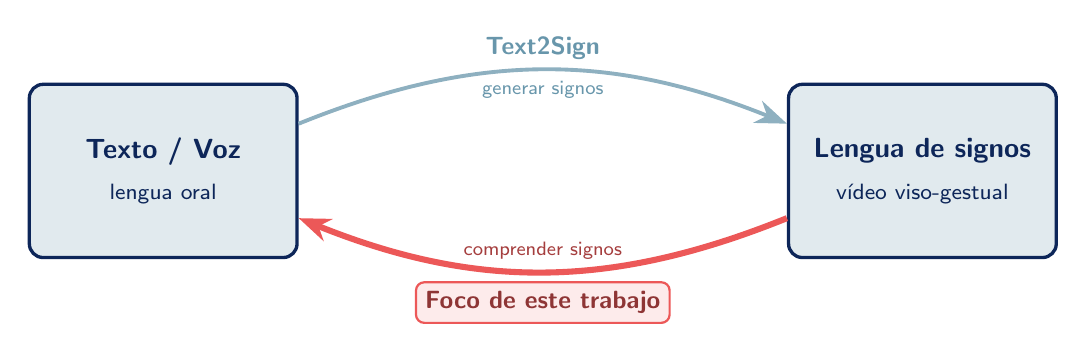
\begin{tikzpicture}[
    font=\sffamily,
    modal/.style={draw=DarkBlue, very thick, rounded corners=5pt,
        fill=MediumBlue!12, minimum width=3.4cm, minimum height=2.2cm,
        align=center, text=DarkBlue},
]

\node[modal] (text) {\textbf{Texto / Voz}\\[3pt]\footnotesize lengua oral};
\node[modal, right=6.2cm of text] (sign) {\textbf{Lengua de signos}\\[3pt]\footnotesize vídeo viso-gestual};

% Text2Sign (arriba, atenuado)
\draw[-{Stealth[length=4mm]}, line width=1.4pt, MediumBlue!45]
    ([yshift=6mm]text.east) to[bend left=22]
    node[above, font=\sffamily\small, text=MediumBlue!60] {\textbf{Text2Sign}}
    node[below, font=\sffamily\scriptsize, text=MediumBlue!60] {generar signos}
    ([yshift=6mm]sign.west);

% Sign2Text (abajo, destacado)
\draw[-{Stealth[length=4mm]}, line width=2.2pt, MediumRed]
    ([yshift=-6mm]sign.west) to[bend left=22]
    node[below, font=\sffamily\bfseries, text=MediumRed] {Sign2Text}
    node[above, font=\sffamily\scriptsize, text=MediumRed!70!black] {comprender signos}
    ([yshift=-6mm]text.east);

% foco del trabajo
\node[draw=MediumRed, thick, rounded corners=3pt, fill=MediumRed!12,
      text=MediumRed!60!black, font=\sffamily\small,
      below=1.4cm of $(text)!0.5!(sign)$] (focus)
    {\textbf{Foco de este trabajo}};

\end{tikzpicture}
\end{document}
